\section{\texorpdfstring{ASIC SkyWater 130\,nm \& LibreLane}{ASIC SkyWater 130nm \& LibreLane}}

\subsection{Cấu hình dự án}
\begin{figure}[H]
    \centering
    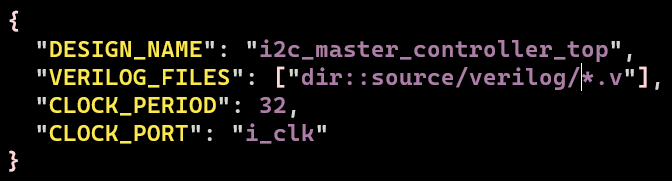
\includegraphics[width=0.88\textwidth,keepaspectratio]{figures/i2c_from_docx/config_json.png}
    \caption{Minh họa file cấu hình (ví dụ \texttt{config.json}) cho luồng LibreLane}
    \label{fig:config_json}
\end{figure}

Từ Hình \ref{fig:config_json} có thể đọc trực tiếp các tham số cấu hình quan trọng:
\begin{itemize}[leftmargin=1.2cm]
    \item \texttt{DESIGN\_NAME}: \texttt{i2c\_master\_controller\_top}.
    \item \texttt{VERILOG\_FILES}: lấy từ thư mục \texttt{source/verilog/*.v}.
    \item \texttt{CLOCK\_PORT}: \texttt{i\_clk}.
    \item \texttt{CLOCK\_PERIOD}: 32 (đặt theo chu kỳ clock hệ thống trong flow).
\end{itemize}

\subsection{Layout và Routing GUI}
\begin{figure}[H]
    \centering
    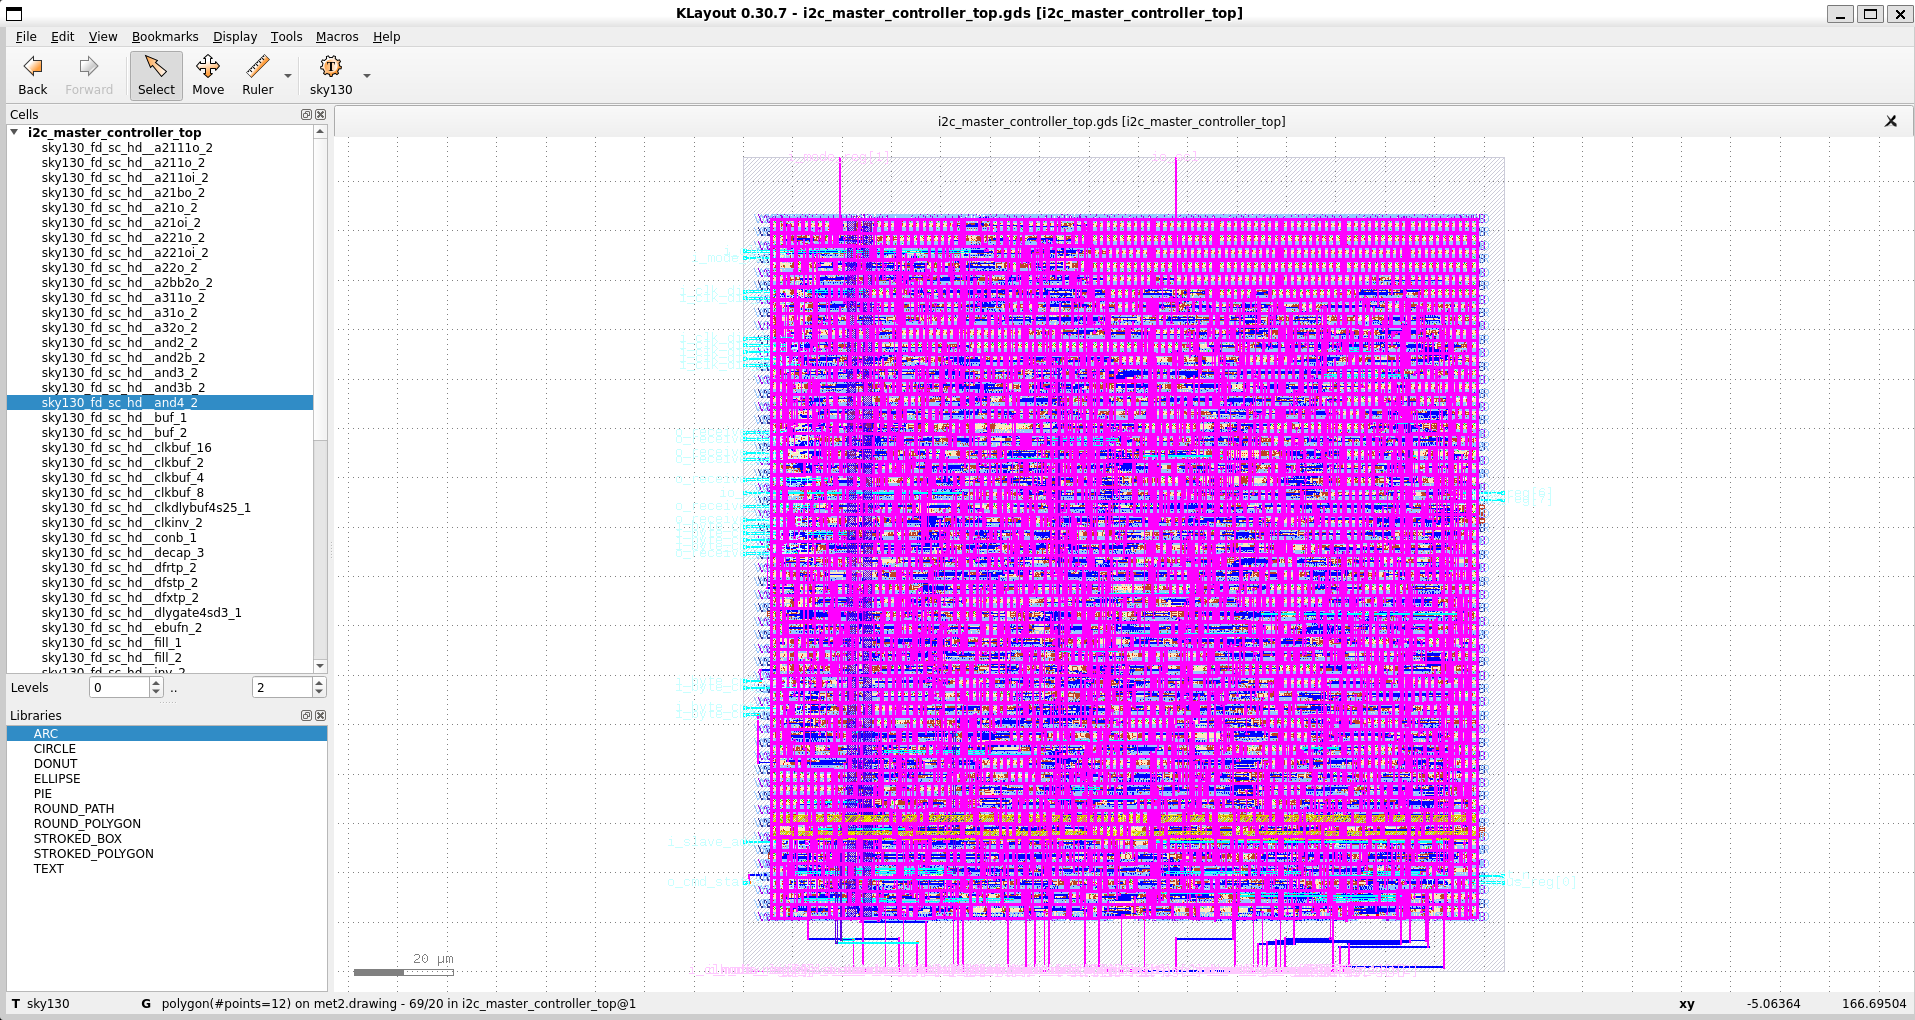
\includegraphics[width=0.95\textwidth,keepaspectratio]{figures/i2c_from_docx/klayout_gui.png}
    \caption{KLayout GUI: xem GDS}
    \label{fig:klayout}
\end{figure}

\begin{figure}[H]
    \centering
    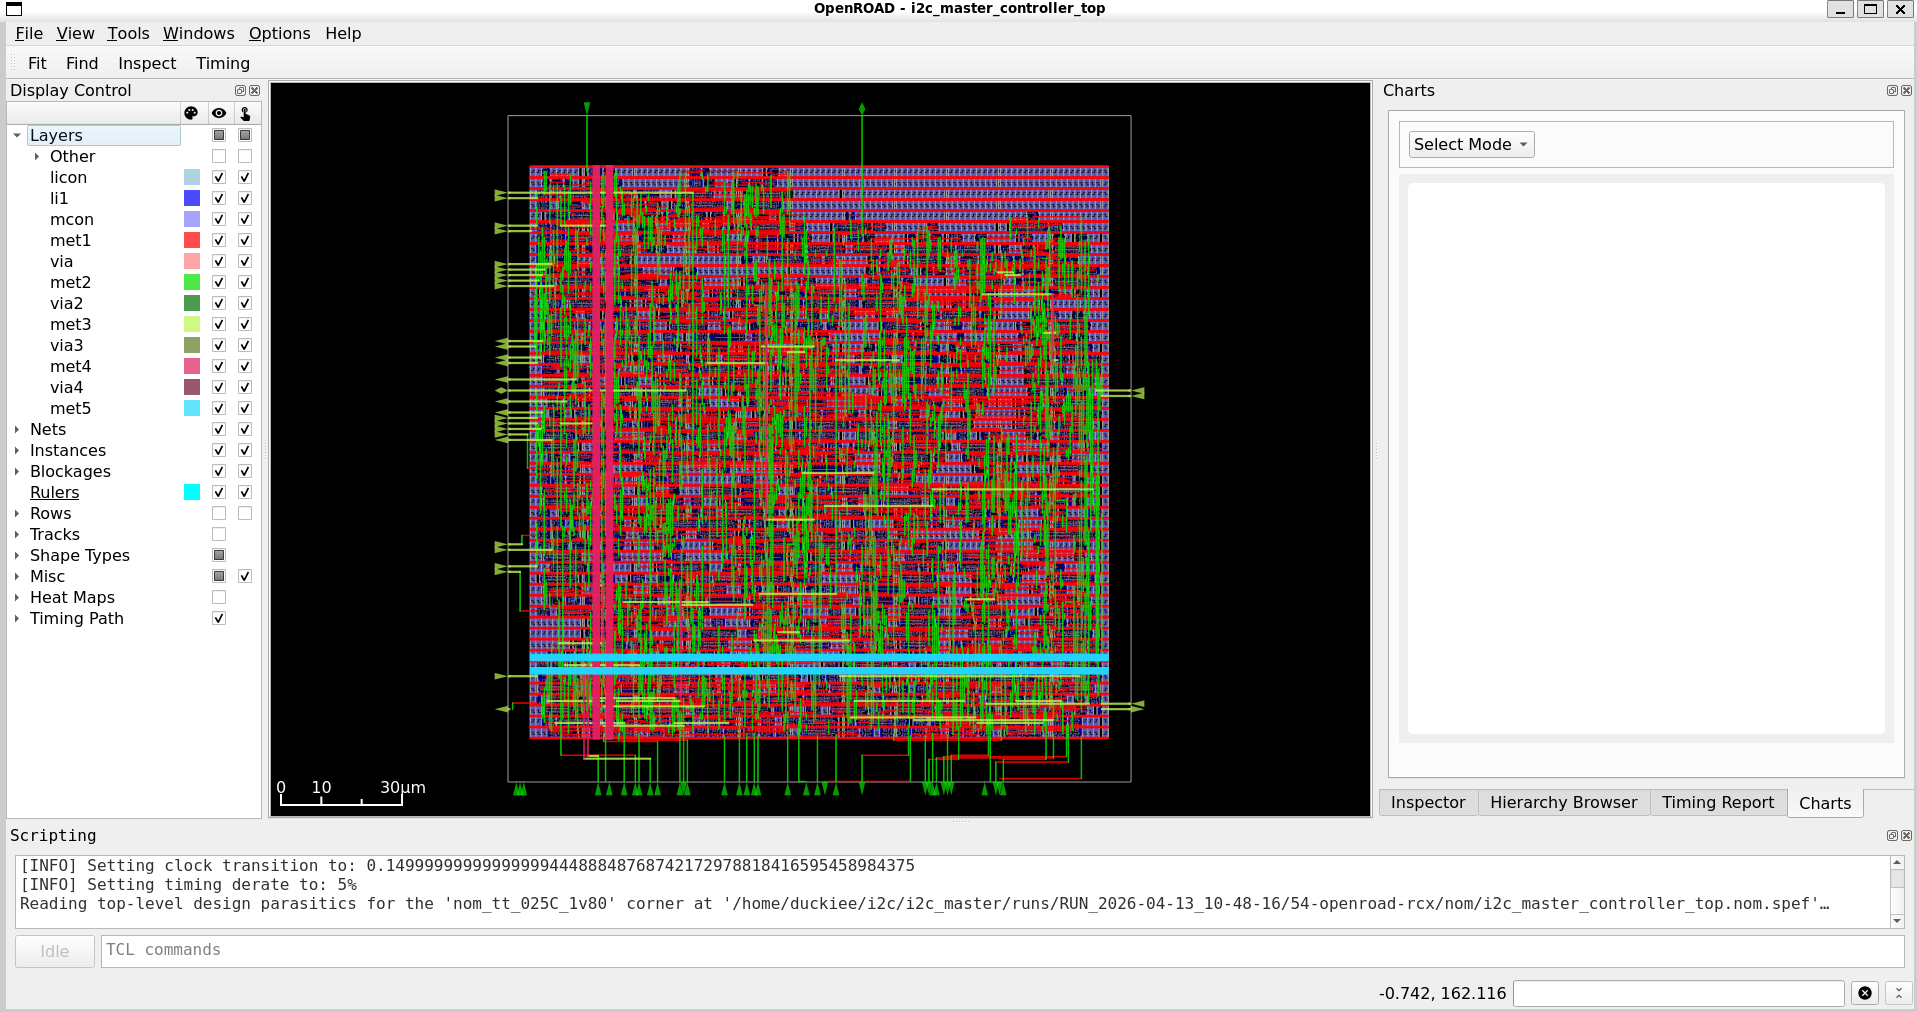
\includegraphics[width=0.95\textwidth,keepaspectratio]{figures/i2c_from_docx/openroad_gui.png}
    \caption{OpenROAD GUI: routing map}
    \label{fig:openroad}
\end{figure}

\subsection{Các bước chạy (run steps) và dấu mốc kiểm chứng}
\begin{figure}[H]
    \centering
    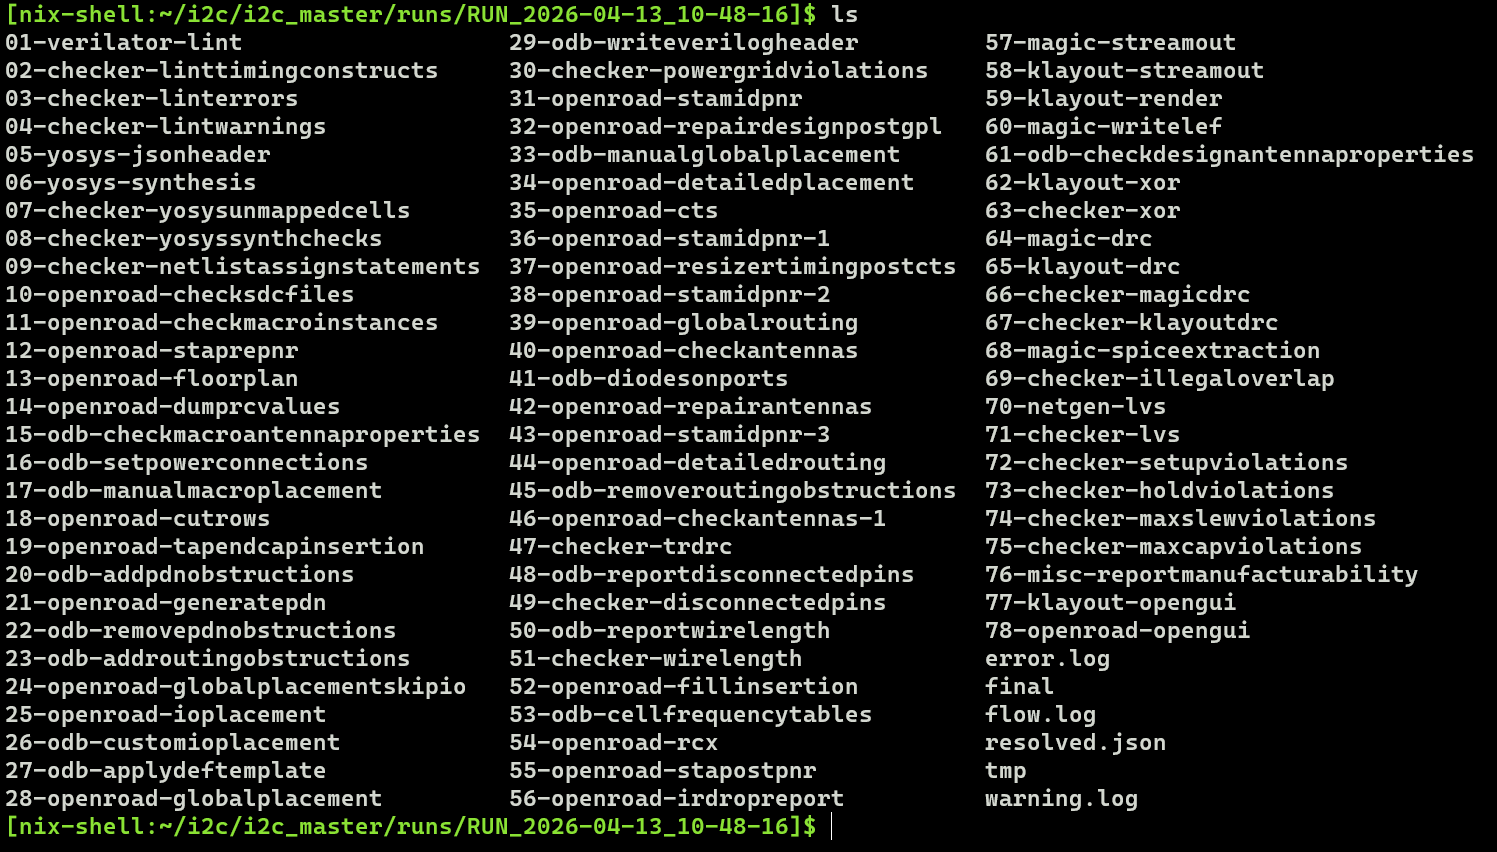
\includegraphics[width=0.95\textwidth,keepaspectratio]{figures/i2c_from_docx/run_steps.png}
    \caption{Danh sách run steps của LibreLane (ví dụ một run với nhiều bước)}
    \label{fig:run_steps}
\end{figure}

Hình \ref{fig:run_steps} minh họa pipeline LibreLane với hơn 75 bước: từ tổng hợp/placement/CTS/routing cho đến các bước hậu PnR và sign-off (antenna, DRC, LVS, STA). Điểm quan trọng khi viết báo cáo là chỉ ra được \textbf{các checkpoint có thể kiểm tra được} thay vì chỉ nói ``đã chạy''.

\subsection{Kết quả tổng hợp \& ký duyệt (trích số liệu từ run)}
\footnote{Nguồn số liệu kết quả: file \texttt{figures/metrics.csv} và \texttt{figures/summary.rpt} do LibreLane/OpenROAD flow sinh ra trong quá trình chạy.}

\begin{table}[H]
    \centering
    \caption{Tóm tắt QoR (theo \texttt{metrics.csv})}
    \label{tab:qor_metrics}
    \begin{tabularx}{\textwidth}{|l|X|}
        \hline
        \textbf{Chỉ số} & \textbf{Giá trị} \\
        \hline
        Instance count & 3281 \\
        \hline
        Stdcell count / area & 1352 / 13955.9\,\(\mu m^2\) \\
        \hline
        Core area / die area & 20234.4\,\(\mu m^2\) / 25433.9\,\(\mu m^2\) \\
        \hline
        Utilization (stdcell) & 0.689711 \\
        \hline
        Total power & 0.0005877 (internal 0.0004523, switching 0.0001354, leakage \(2.17\times 10^{-8}\)) \\
        \hline
        DRC / LVS / Antenna violations & 0 / 0 / 0 \\
        \hline
    \end{tabularx}
\end{table}

\begin{table}[H]
    \centering
    \caption{Tóm tắt STA multi-corner (theo \texttt{summary.rpt})}
    \label{tab:sta_summary_rpt}
    \begin{tabularx}{\textwidth}{|l|c|c|c|c|}
        \hline
        \textbf{Corner} & \textbf{Hold worst slack} & \textbf{Hold vio} & \textbf{Setup worst slack} & \textbf{Setup vio} \\
        \hline
        Overall & 0.1077 & 0 & 20.6567 & 0 \\
        \hline
        nom\_tt\_025C\_1v80 & 0.3115 & 0 & 23.2111 & 0 \\
        \hline
        nom\_ss\_100C\_1v60 & 0.8392 & 0 & 20.7446 & 0 \\
        \hline
        nom\_ff\_n40C\_1v95 & 0.1092 & 0 & 24.1089 & 0 \\
        \hline
    \end{tabularx}
\end{table}

Từ Bảng \ref{tab:sta_summary_rpt} có thể kết luận: \textbf{không có vi phạm setup/hold} ở các corner được báo cáo (TNS = 0, violation count = 0), tức thiết kế \textbf{đạt timing} theo cấu hình clock trong flow.

\subsection{Kết quả log sign-off (trích từ log/report của một run)}
\footnote{Nguồn kết quả log: các log/report do LibreLane/OpenROAD/Magic/Netgen sinh ra trong một lần chạy (run). Phần này trích trực tiếp các dòng kết luận quan trọng.}

\begin{table}[H]
    \centering
    \caption{Tóm tắt kết quả log sign-off (trích)}
    \label{tab:signoff_log_summary}
    \begin{tabularx}{\textwidth}{|l|X|}
        \hline
        \textbf{Hạng mục} & \textbf{Kết quả log (trích)} \\
        \hline
        STA checker & ``No setup violations found''; ``No hold violations found''. \\
        \hline
        STA summary & Setup/Hold violation count = 0; TNS = 0 ở các corner báo cáo (xem Bảng \ref{tab:sta_summary_rpt}). \\
        \hline
        DRC (Magic) & COUNT = 0. \\
        \hline
        LVS (Netgen) & ``Final result: Circuits match uniquely.'' \\
        \hline
        Antenna & Bảng tóm tắt không có net/pin vi phạm (không liệt kê dòng nào trong summary). \\
        \hline
        Max slew checker & Có ghi nhận max slew violation ở các corner SS (slow/\(T\) cao): nom\_ss, min\_ss, max\_ss; cần tối ưu thêm nếu yêu cầu sign-off strict. \\
        \hline
    \end{tabularx}
\end{table}

Như vậy, báo cáo tách bạch hai ý: \textbf{timing setup/hold đạt} (không violation), nhưng \textbf{slew vẫn có vi phạm} ở corner SS; đây là phần cần xử lý nếu nâng tiêu chí từ ``minh họa flow'' lên ``sign-off nghiêm ngặt''.

\subsection{Sign-off (DRC/LVS/STA/IPVT)}
\begin{figure}[H]
    \centering
    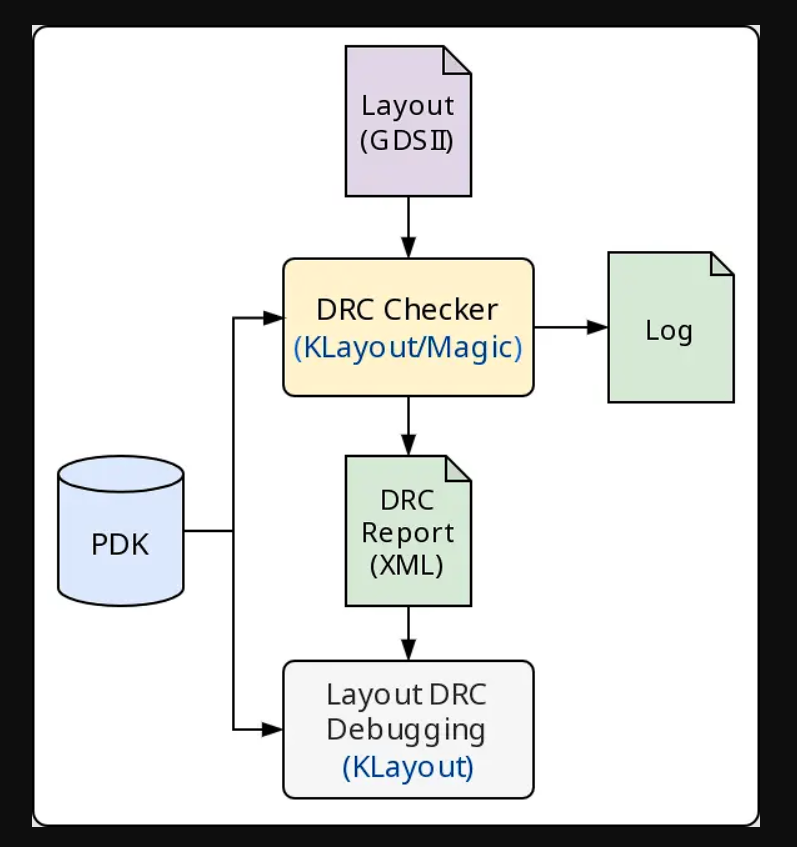
\includegraphics[width=0.88\textwidth,keepaspectratio]{figures/i2c_from_docx/drc_flow.png}
    \caption{DRC Flow}
    \label{fig:drc_flow}
\end{figure}

Hình \ref{fig:drc_flow} mô tả luồng DRC: \textbf{Layout (GDSII)} và \textbf{PDK} được đưa vào \textbf{DRC Checker (KLayout/Magic)} để sinh \textbf{Log} và \textbf{DRC Report (XML)}; XML tiếp tục được nạp vào KLayout để debug vi phạm theo marker.

\begin{figure}[H]
    \centering
    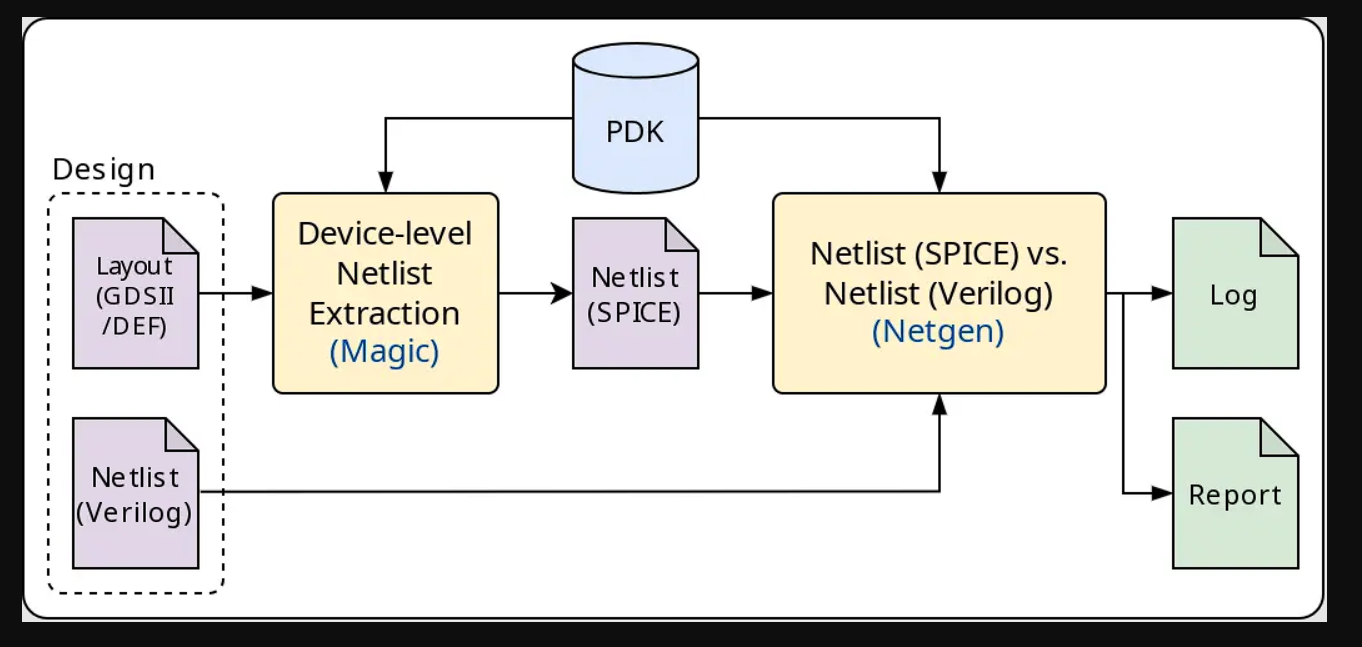
\includegraphics[width=0.88\textwidth,keepaspectratio]{figures/i2c_from_docx/lvs_flow.png}
    \caption{LVS Flow}
    \label{fig:lvs_flow}
\end{figure}

Theo Hình \ref{fig:lvs_flow}, LVS gồm 2 nhánh đầu vào: (1) layout (GDSII/DEF) và (2) netlist Verilog. Layout được Magic \textbf{trích xuất netlist mức thiết bị} thành SPICE. Sau đó Netgen so sánh \textbf{SPICE vs Verilog} để xuất \textbf{Log} và \textbf{Report}.

\begin{figure}[H]
    \centering
    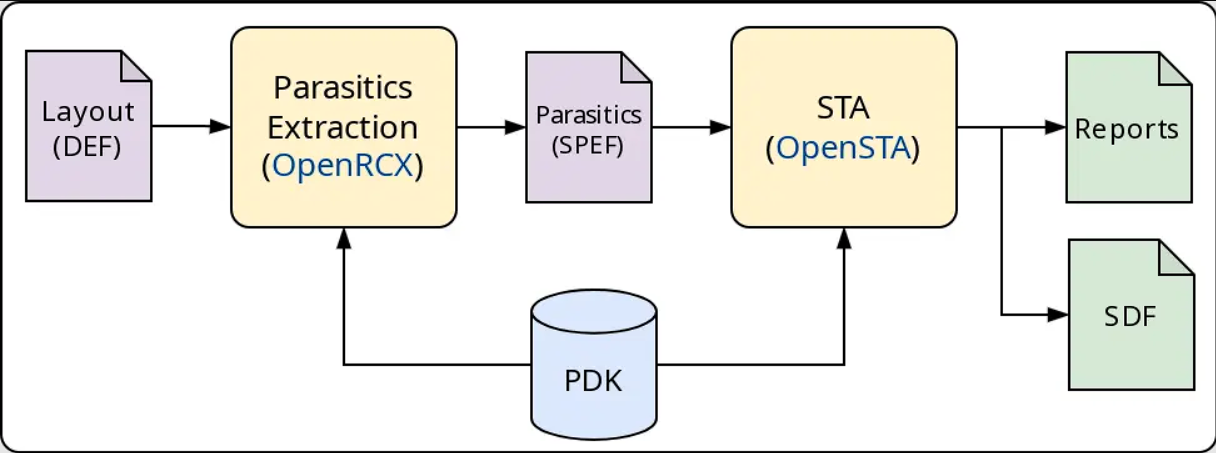
\includegraphics[width=0.88\textwidth,keepaspectratio]{figures/i2c_from_docx/sta_flow.png}
    \caption{STA Flow}
    \label{fig:sta_flow}
\end{figure}

Hình \ref{fig:sta_flow} mô tả STA: từ layout DEF và PDK, OpenRCX trích xuất parasitic tạo SPEF; OpenSTA dùng SPEF + thư viện/constraint để xuất báo cáo timing và file SDF phục vụ mô phỏng hậu layout.

\begin{figure}[H]
    \centering
    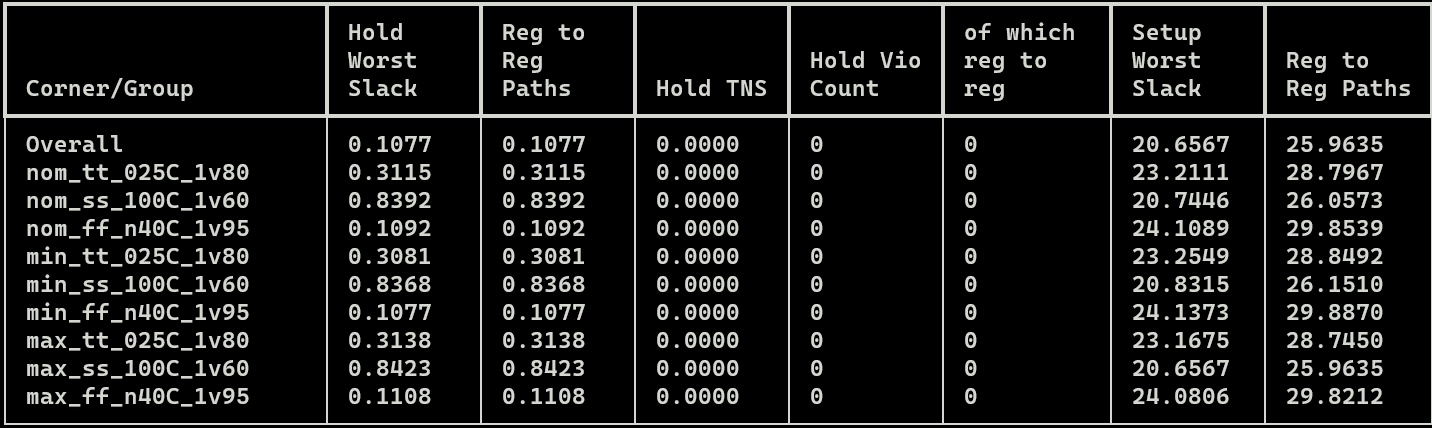
\includegraphics[width=0.95\textwidth,keepaspectratio]{figures/i2c_from_docx/sta_summary_1.png}
    \caption{Ví dụ STA summary (phần 1)}
    \label{fig:sta_summary_1}
\end{figure}

\begin{figure}[H]
    \centering
    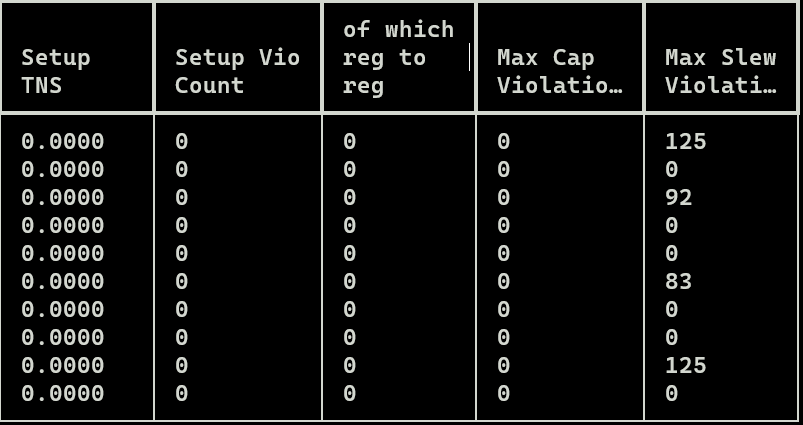
\includegraphics[width=0.95\textwidth,keepaspectratio]{figures/i2c_from_docx/sta_summary_2.png}
    \caption{Ví dụ STA summary (phần 2)}
    \label{fig:sta_summary_2}
\end{figure}

Hai hình \ref{fig:sta_summary_1}--\ref{fig:sta_summary_2} là kiểu báo cáo mà thầy thường muốn thấy: có \textbf{WNS/TNS} (worst/total negative slack) cho setup/hold, cùng các thống kê vi phạm để kết luận ``đạt timing'' ở corner đang xét.

\begin{figure}[H]
    \centering
    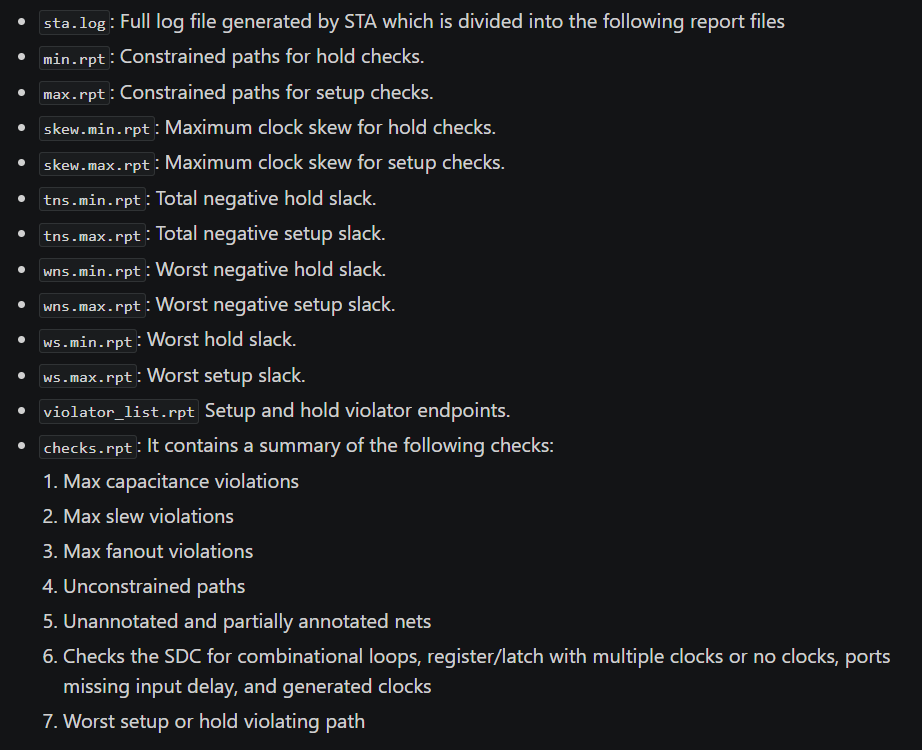
\includegraphics[width=0.95\textwidth,keepaspectratio]{figures/i2c_from_docx/IPVT_corner_explain.png}
    \caption{Ý nghĩa các Corner IPVT}
    \label{fig:ipvt}
\end{figure}

Hình \ref{fig:ipvt} liệt kê nhóm báo cáo STA thường gặp (ví dụ \texttt{min.rpt}, \texttt{max.rpt}, \texttt{wns.*}, \texttt{tns.*}, \texttt{skew.*}, \texttt{violator\_list.rpt}) và các hạng mục kiểm tra tổng hợp trong \texttt{checks.rpt} (capacitance, slew, fanout, unconstrained paths, SDC sanity, v.v.).

\begin{figure}[H]
    \centering
    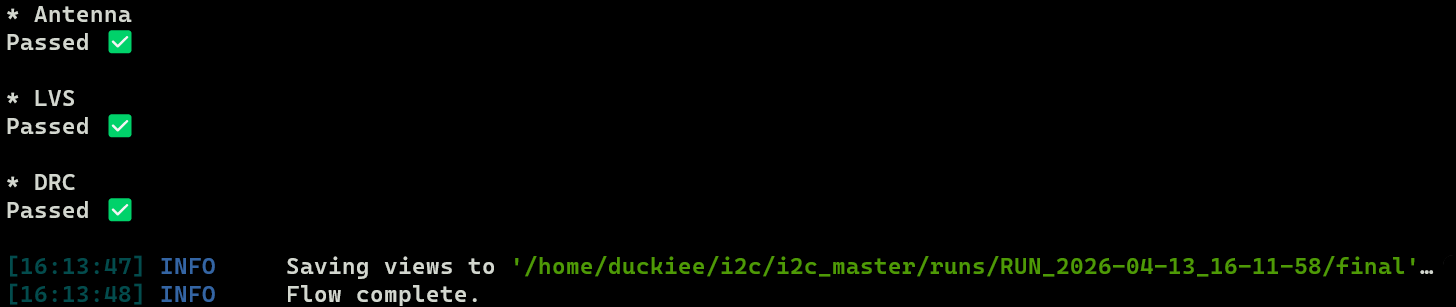
\includegraphics[width=0.88\textwidth,keepaspectratio]{figures/i2c_from_docx/pass_signoff.png}
    \caption{Pass sign-off}
    \label{fig:pass_signoff}
\end{figure}

Từ log trong Hình \ref{fig:pass_signoff} có thể thấy trạng thái \textbf{Antenna/LVS/DRC đều Passed} và flow kết thúc với thư mục \texttt{.../runs/.../final}.

\footnote{Tham chiếu flow/tool: Efabless LibreLane documentation (OpenROAD/OpenSTA/OpenRCX, KLayout/Magic/Netgen) --- xem phần References của báo cáo.}

